% Options for packages loaded elsewhere
\PassOptionsToPackage{unicode}{hyperref}
\PassOptionsToPackage{hyphens}{url}
%
\documentclass[
]{article}
\usepackage{amsmath,amssymb}
\usepackage{lmodern}
\usepackage{iftex}
\ifPDFTeX
  \usepackage[T1]{fontenc}
  \usepackage[utf8]{inputenc}
  \usepackage{textcomp} % provide euro and other symbols
\else % if luatex or xetex
  \usepackage{unicode-math}
  \defaultfontfeatures{Scale=MatchLowercase}
  \defaultfontfeatures[\rmfamily]{Ligatures=TeX,Scale=1}
\fi
% Use upquote if available, for straight quotes in verbatim environments
\IfFileExists{upquote.sty}{\usepackage{upquote}}{}
\IfFileExists{microtype.sty}{% use microtype if available
  \usepackage[]{microtype}
  \UseMicrotypeSet[protrusion]{basicmath} % disable protrusion for tt fonts
}{}
\makeatletter
\@ifundefined{KOMAClassName}{% if non-KOMA class
  \IfFileExists{parskip.sty}{%
    \usepackage{parskip}
  }{% else
    \setlength{\parindent}{0pt}
    \setlength{\parskip}{6pt plus 2pt minus 1pt}}
}{% if KOMA class
  \KOMAoptions{parskip=half}}
\makeatother
\usepackage{xcolor}
\usepackage[margin=1in]{geometry}
\usepackage{longtable,booktabs,array}
\usepackage{calc} % for calculating minipage widths
% Correct order of tables after \paragraph or \subparagraph
\usepackage{etoolbox}
\makeatletter
\patchcmd\longtable{\par}{\if@noskipsec\mbox{}\fi\par}{}{}
\makeatother
% Allow footnotes in longtable head/foot
\IfFileExists{footnotehyper.sty}{\usepackage{footnotehyper}}{\usepackage{footnote}}
\makesavenoteenv{longtable}
\usepackage{graphicx}
\makeatletter
\def\maxwidth{\ifdim\Gin@nat@width>\linewidth\linewidth\else\Gin@nat@width\fi}
\def\maxheight{\ifdim\Gin@nat@height>\textheight\textheight\else\Gin@nat@height\fi}
\makeatother
% Scale images if necessary, so that they will not overflow the page
% margins by default, and it is still possible to overwrite the defaults
% using explicit options in \includegraphics[width, height, ...]{}
\setkeys{Gin}{width=\maxwidth,height=\maxheight,keepaspectratio}
% Set default figure placement to htbp
\makeatletter
\def\fps@figure{htbp}
\makeatother
\setlength{\emergencystretch}{3em} % prevent overfull lines
\providecommand{\tightlist}{%
  \setlength{\itemsep}{0pt}\setlength{\parskip}{0pt}}
\setcounter{secnumdepth}{-\maxdimen} % remove section numbering
\usepackage{booktabs}
\usepackage{longtable}
\usepackage{array}
\usepackage{multirow}
\usepackage{wrapfig}
\usepackage{float}
\usepackage{colortbl}
\usepackage{pdflscape}
\usepackage{tabu}
\usepackage{threeparttable}
\usepackage{threeparttablex}
\usepackage[normalem]{ulem}
\usepackage{makecell}
\usepackage{xcolor}
\ifLuaTeX
  \usepackage{selnolig}  % disable illegal ligatures
\fi
\IfFileExists{bookmark.sty}{\usepackage{bookmark}}{\usepackage{hyperref}}
\IfFileExists{xurl.sty}{\usepackage{xurl}}{} % add URL line breaks if available
\urlstyle{same} % disable monospaced font for URLs
\hypersetup{
  pdftitle={Convergence Concepts},
  hidelinks,
  pdfcreator={LaTeX via pandoc}}

\title{Convergence Concepts}
\author{}
\date{\vspace{-2.5em}}

\begin{document}
\maketitle

\hypertarget{limit-theory}{%
\section{Limit Theory}\label{limit-theory}}

\hypertarget{convergence-in-probability}{%
\subsection{Convergence in
Probability}\label{convergence-in-probability}}

\hypertarget{definition}{%
\subsubsection{Definition}\label{definition}}

We saw that the estimator of \(p\), \(\hat{p}\), from the Binomial
example seemed to be observed closer and closer to \(p\) for larger
sample sizes. Additionally, we saw a good large-sample distribution for
\(\hat{p}\) is
\[\hat{p}\stackrel{\bullet}\sim N\left(p, \frac{p(1-p)}{n}\right)\]

Does this large-sample distribution support the `convergence' of
\(\hat{p}\) to \(p\) idea?

More formally, we're going to take on the idea of \textbf{convergence in
probability to a constant}. First, let's define convergence in
probability generally.

\begin{description}
\tightlist
\item[Convergence in Probability]
A sequence of RVs \(Y_1,...,Y_n,...\) converges in probability to a RV
\(Y\) if for every \(\epsilon>0\)
\[\lim_{n\rightarrow\infty}P(|Y_n-Y|\geq \epsilon)=0 \iff 
\lim_{n\rightarrow\infty}P(|Y_n-Y|<\epsilon)=1\] This is denoted as
\[Y_n\stackrel{p}{\rightarrow}Y\]
\end{description}

We'll mostly care about convergence in probability to a constant, call
it \(c\). We can see the definition in this case can be simplied to the
following:
\[\lim_{n\rightarrow\infty}P(|Y_n-c|< \epsilon)=\lim_{n\rightarrow\infty}P(-\epsilon < Y_n-c<\epsilon) =  \lim_{n\rightarrow\infty}P(c-\epsilon < Y_n<c+\epsilon)=1\]
\(Y_n\stackrel{p}\rightarrow c\) if the \emph{probability} we observe
\(Y_n\) close to \(c\) goes to 1 in the limit.

\textbf{Example} - We can visualize this idea.

Assume that \(Y_i\stackrel{iid}\sim N(0,1)\). Let's investigate the
behavior of \[X = \frac{1}{n^2}\sum_{i=1}^{n}Y_i\] To put this in the
context of the definition, let's refer to \(X\) explicitly as a function
of \(n\): \[X_n = \frac{1}{n^2}\sum_{i=1}^{n}Y_i\] We want to understand
the behavior of \(X_n\) as n grows. We'll see that
\(X_n\stackrel{p}\rightarrow 0\), which implies that for any
\(\epsilon>0\) we have
\[\lim_{n\rightarrow\infty}P(-\epsilon < X_n < \epsilon) =0\]

To visualize this, we can consider \textbf{sample paths} of \(X_n\).
That is, we can look at a particular sequence of \(y_i\)'s that will
generate a sequence of \(x\) and see how the values change.

Consider the following 6 values randomly sampled from a \(N(0,1)\) and
the corresponding sequence of \(x_n\) values.

\begin{longtable}[]{@{}
  >{\raggedright\arraybackslash}p{(\columnwidth - 2\tabcolsep) * \real{0.5625}}
  >{\raggedright\arraybackslash}p{(\columnwidth - 2\tabcolsep) * \real{0.4375}}@{}}
\toprule()
\begin{minipage}[b]{\linewidth}\raggedright
\(y\) sequence
\end{minipage} & \begin{minipage}[b]{\linewidth}\raggedright
\(x\) sequence
\end{minipage} \\
\midrule()
\endhead
\(y_1\) = -0.6264538 & \(x_1\) = -0.6264538\(/1^2\) = -0.6264538 \\
\(y_2\) = 0.1836433 & \(x_2\) = (-0.6264538+0.1836433)\(/2^2\) =
-0.1107026 \\
\(y_3\) = -0.8356286 & \(x_3\) =
(-0.6264538+0.1836433+-0.8356286)\(/3^2\) = -0.1420488 \\
\(y_4\) = 1.5952808 & \(x_4\) = (-0.6264538+\ldots+1.5952808)\(/4^2\) =
0.0198026 \\
\(y_5\) = 0.3295078 & \(x_5\) = (-0.6264538+\ldots+0.3295078)\(/5^2\) =
0.025854 \\
\(y_6\) = -0.8204684 & \(x_6\) = (-0.6264538+\ldots+-0.8204684)\(/6^2\)
= -0.0048366 \\
\bottomrule()
\end{longtable}

If we consider multiple sample paths, then convergence in probability to
0 of this sequence implies that the proportion of sample paths outside
of \(\pm \epsilon\) should go to zero.

Let's plot our sample path with an \(\epsilon = 0.05\):

\includegraphics{ConvergenceConceptsNotesToPDF2_files/figure-latex/unnamed-chunk-2-1.pdf}

Now let's add 9 more sample paths:

\includegraphics{ConvergenceConceptsNotesToPDF2_files/figure-latex/unnamed-chunk-3-1.pdf}

What we hope to see is that the proportion of lines falling outside of
the \(\epsilon\) bars goes to 0!

\begin{table}

\caption{\label{tab:unnamed-chunk-4}<center> Probability for 10 Simuations 
                  with sample size 6 </center>}
\centering
\begin{tabu} to \linewidth {>{\raggedright}X>{\raggedright}X>{\raggedright}X>{\raggedright}X>{\raggedright}X>{\raggedright}X>{\raggedright}X}
\hline
  & X1 & X2 & X3 & X4 & X5 & X6\\
\hline
Sample Path 1 & \textcolor{black}{-0.63} & \textcolor{black}{-0.11} & \textcolor{black}{-0.14} & \textcolor{black}{0.02} & \textcolor{black}{0.03} & \textcolor{black}{0}\\
\hline
Sample Path 2 & \textcolor{red}{0.49} & \textcolor{red}{0.31} & \textcolor{red}{0.2} & \textcolor{red}{0.09} & \textcolor{red}{0.12} & \textcolor{red}{0.09}\\
\hline
Sample Path 3 & \textcolor{black}{-0.62} & \textcolor{black}{-0.71} & \textcolor{black}{-0.19} & \textcolor{black}{-0.11} & \textcolor{black}{-0.07} & \textcolor{black}{-0.02}\\
\hline
Sample Path 4 & \textcolor{red}{0.82} & \textcolor{red}{0.35} & \textcolor{red}{0.26} & \textcolor{red}{0.19} & \textcolor{red}{0.13} & \textcolor{black}{0.03}\\
\hline
Sample Path 5 & \textcolor{red}{0.62} & \textcolor{red}{0.14} & \textcolor{red}{0.05} & \textcolor{black}{-0.07} & \textcolor{black}{-0.06} & \textcolor{black}{-0.03}\\
\hline
Sample Path 6 & \textcolor{red}{1.36} & \textcolor{red}{0.31} & \textcolor{red}{0.18} & \textcolor{red}{0.1} & \textcolor{black}{0.01} & \textcolor{black}{-0.01}\\
\hline
Sample Path 7 & \textcolor{black}{-0.39} & \textcolor{black}{-0.11} & \textcolor{red}{0.07} & \textcolor{red}{0.09} & \textcolor{red}{0.05} & \textcolor{black}{0.03}\\
\hline
Sample Path 8 & \textcolor{red}{0.7} & \textcolor{red}{0.31} & \textcolor{red}{0.06} & \textcolor{black}{-0.01} & \textcolor{black}{0.01} & \textcolor{black}{0.03}\\
\hline
Sample Path 9 & \textcolor{black}{-0.11} & \textcolor{red}{0.19} & \textcolor{red}{0.13} & \textcolor{black}{0.03} & \textcolor{black}{0.04} & \textcolor{black}{-0.01}\\
\hline
Sample Path 10 & \textcolor{red}{1.43} & \textcolor{red}{0.85} & \textcolor{red}{0.34} & \textcolor{red}{0.13} & \textcolor{red}{0.1} & \textcolor{red}{0.07}\\
\hline
\cellcolor{lightblue}{\textcolor{black}{\textbf{Probability}}} & \cellcolor{lightblue}{\textcolor{black}{\textbf{1}}} & \cellcolor{lightblue}{\textcolor{black}{\textbf{1}}} & \cellcolor{lightblue}{\textcolor{black}{\textbf{0.9}}} & \cellcolor{lightblue}{\textcolor{black}{\textbf{0.7}}} & \cellcolor{lightblue}{\textcolor{black}{\textbf{0.5}}} & \cellcolor{lightblue}{\textcolor{black}{\textbf{0.2}}}\\
\hline
\end{tabu}
\end{table}

\textbf{Example} - Suppose we have a random sample from a Normal
distribution with mean 10 and standard deviation 1. What do you think
\(W = (\bar{Y})^2\) converges to in probability? Take an educated guess
and use the app below to explore!

\begin{itemize}
\tightlist
\item
  Select the value c that you guess \(W\) converges to in probability.
\item
  Choose a sample size to go up to (start smaller and then get larger
  once you have a good idea).
\item
  Select an \(\epsilon\) range.
\item
  Look for the proportion of lines (50 sample paths are generated)
  falling outside of the \(\epsilon\) bars to go to 0!
\end{itemize}

\vspace{4in}

\hypertarget{inequalities}{%
\subsubsection{Inequalities}\label{inequalities}}

To prove convergence in probability, we'll sometimes rely on some very
famous inequalities. These will help us to show the probability goes to
0 or 1.

\begin{description}
\tightlist
\item[Markov's Inequality]
If \(X\) is a nonnegative RV (support has no negative values) for which
\(E(X)\) exists, then for \(t>0\) \[P(X\geq t)\leq \frac{E(X)}{t}\]
\end{description}

Example: If \(X\sim exp(1)\) then \(P(X\geq t)=e^{-t}\) and
\(E(X)/t=1/t\).

\begin{center}\includegraphics[width=550px]{ConvergenceConceptsNotesToPDF2_files/figure-latex/unnamed-chunk-5-1} \end{center}

\begin{description}
\tightlist
\item[Chebychev's Inequality]
Let \(X\) be a RV with mean = \(\mu\) and variance = \(\sigma^2\), then
for \(t>0\) \[P(|X-\mu|\geq t)\leq \frac{\sigma^2}{t^2}\]
\end{description}

Example: If \(t=\sigma k\) for \(k>0\), we can apply Chebychev's to get
\[P\left(|X-\mu|\geq k\sigma\right)\leq \frac{\sigma^2}{k^2\sigma^2}=\frac{1}{k^2}\]
For \(k=2\) we have \(P\left(|X-\mu|\geq 2\sigma\right)\leq 1/4\).

Practically, what can we take home from this?

\begin{itemize}
\tightlist
\item
  At least 75\% of a RVs distribution lies within 2 standard deviations
  of the mean (if these moments exist)
\item
  Regardless of distribution! (if moments exist)
\item
  If \(X\sim N(\mu,\sigma^2)\) we know
  \(P(|X-\mu|\geq 2\sigma)\approx 0.05\). The bound isn't always very
  tight!
\end{itemize}

\hypertarget{wlln}{%
\subsubsection{WLLN}\label{wlln}}

One of the most important results regarding convergence in probability
is called the Law of Large Numbers (LLN).

\begin{description}
\tightlist
\item[(Weak) Law of Large Numbers (WLLN)]
Suppose \(Y_i\stackrel{iid}\sim f\) where the mean and variance of
\(Y_i\) exist. Then
\[\bar{Y}=\frac{1}{n}\sum_{i=1}^{n}Y_i\stackrel{p}\rightarrow E(Y)=\mu\]
\end{description}

\begin{itemize}
\tightlist
\item
  Big picture goal is to estimate parameters such as \(\mu\)
\item
  If we get a RS we know that \(\bar{Y}\) will be a `close' to \(\mu\)
  for `large' samples
\item
  Applies to the \textbf{average of any independent random variables
  with the same finite mean}
\end{itemize}

Note that the variance assumption is actually not needed but will help
us facilitate an easy proof. Let's use our inequalities to prove this
result!

\textbf{Example} - Let \(Y_i\stackrel{iid}{\sim}N(\mu, \sigma^2)\). What
does \(\bar{Y}\) converge to? What does
\(\frac{1}{n}\sum_{i=1}^{n}Y_i^2\) converge to?

\hypertarget{continuity-theorems}{%
\subsubsection{Continuity Theorems}\label{continuity-theorems}}

The WLLN is also quite useful when combined with the continuity theorem.

\begin{description}
\tightlist
\item[Continuity Theorem]
If \(Y_1,Y_2,Y_3,...\) converge to \(Y\) and \(g()\) is a continuous
function then \(g(Y_1),g(Y_2),g(Y_3)...\) converge to \(g(Y)\).
\end{description}

\textbf{Example (exploration example proved)} - Suppose we have a random
sample from a Normal distribution with mean 10 and standard deviation 1.
Consider \(W = (\bar{Y})^2\). What does this converge to in probability?

Note: The continuity theorem also works for convergence in distribution!

\textbf{Example} - Suppose that
\(Y_i\stackrel{iid}\sim gamma(\alpha, \lambda)\). We have that
\[\frac{\bar{Y}-\alpha/\lambda}{\frac{\alpha}{\lambda^2\sqrt{n}}}\stackrel{d}\rightarrow Z\]
where \(Z\sim N(0,1)\). By the continuity theorem we have that
\[\left(\frac{\bar{Y}-\alpha/\lambda}{\frac{\alpha}{\lambda^2\sqrt{n}}}\right)^2\stackrel{d}\rightarrow Z^2\]
and recall that a standard Normal squared is distributed as a
\(\chi^2_1\) or a \(gamma(1/2, 1/2)\).

\hypertarget{other-standard-limit-results-work-too}{%
\paragraph{Other Standard Limit Results Work
Too!}\label{other-standard-limit-results-work-too}}

Most of the common limit theorem ideas from calculus follow here as well
(\(\theta\) and \(\lambda\) are constants below):

\[\mbox{If }Y\stackrel{p}{\rightarrow}\theta, X\stackrel{p}{\rightarrow}\lambda\mbox{ then }Y\pm X\stackrel{p}{\rightarrow}\theta\pm\lambda\]

\textbf{Example} - Consider the `biased' version of the sample variance,
\(S_n^2=\frac{1}{n}\sum_{i=1}^{n}(Y_i-\bar{Y})^2\). Let's show
\(S_n^2\stackrel{p}{\rightarrow}\sigma^2\)

\hypertarget{stackreldrightarrow-stackrelprightarrow-relationship}{%
\subsubsection{\texorpdfstring{\(\stackrel{d}\rightarrow\) \&
\(\stackrel{p}\rightarrow\)
Relationship}{\textbackslash stackrel\{d\}\textbackslash rightarrow \& \textbackslash stackrel\{p\}\textbackslash rightarrow Relationship}}\label{stackreldrightarrow-stackrelprightarrow-relationship}}

Convergence in probability implies convergence in distribution. However,
the converse is not true generally (convegence in distribution does not
imply convergence in probability).

\textbf{Example} - Suppose \(X\sim Beta(2,2)\) then \(1-X\) is also
distributed as Beta(2,2) (recall the symmetry of the Beta distribution
with equal \(\alpha\) and \(\beta\)).

Define a sequence of RVs to be \(X_n=X\) for all \(n\). Then
\(X_n\stackrel{d}{\rightarrow}1-X\sim Beta(2,2)\).

Now consider convergence in probability, does
\(X_n\stackrel{p}{\rightarrow}1-X\)? No! To converge in probability we
need \[P(|X_n-(1-X)|<\epsilon)=P(|X+X_n-1|<\epsilon)\rightarrow 1\] as n
goes to infinity for \textbf{every} \(\epsilon>0\). Pick an
\(\epsilon\), say \(\epsilon = 1/2\). As \(X_n\) is defined as \(X\), we
have

\begin{eqnarray*}
P(|X+X_n-1|<\epsilon)=P(|2X-1|<\epsilon) & = & P((1-\epsilon)/2 < X < (1+\epsilon)/2) < 1\\
                     &= &P(1/4 < X < 3/4) <1
\end{eqnarray*} for all \(n\).

\textbf{Convergence in distribution to a constant} - If
\(Y_n\stackrel{d}{\rightarrow}c\) then \(Y_n\stackrel{p}\rightarrow c\).

Why does it makes sense that convergence in distribution to a constant
implies convergence in probability to that constant? Consider our
example where we look at the maximum from a random sample of \(U(0,1)\)
RVs. Below are plots of the distribution of the sample max for varying
\(n\) values.

\includegraphics{ConvergenceConceptsNotesToPDF2_files/figure-latex/unnamed-chunk-6-1.pdf}

Another really useful theorem relating convergence results is called
Slutsky's Theorem.

\begin{description}
\tightlist
\item[Slutsky's Theorem]
If \(X_n\stackrel{d}\rightarrow X\) and
\(Y_n\stackrel{p}\rightarrow a\), then
\end{description}

\begin{itemize}
\tightlist
\item
  \(X_nY_n\stackrel{d}\rightarrow aX\)
\item
  \(X_n+Y_n\stackrel{d}\rightarrow X+a\)
\end{itemize}

This theorem is extremely useful for creating hypothesis tests and
confidence intervals! Recall the example we talked about when discussing
the importance of the CLT:

\textbf{Example:}

\begin{itemize}
\tightlist
\item
  Suppose we know \(\sigma\) and we want inference for \(\mu\).
\item
  If we have a random sample \(Y_1,...,Y_n\), we know
  \(\bar{Y}\stackrel{\bullet}{\sim}N(\mu,\sigma^2/n)\) (\(\mu\) only
  unknown)
\item
  We can make an approximate claim about \(\mu\) via a confidence
  interval derived from an argument similar to that below:
\end{itemize}

\begin{align*}
P(-1.96<Z<1.96) &= 0.95\\
\Leftrightarrow P\left(-1.96<\frac{\bar{Y}-\mu}{\sigma/\sqrt{n}}<1.96\right) &= 0.95\\
\Leftrightarrow P\left(\bar{Y}-1.96\sigma/\sqrt{n}<\mu<\bar{Y}+1.96\sigma/\sqrt{n}\right) &= 0.95\\
\end{align*}

\begin{itemize}
\tightlist
\item
  That is, there is a 95\% probability the RVs
  \(\bar{Y}-1.96\sigma/\sqrt{n}\) and \(\bar{Y}+1.96\sigma/\sqrt{n}\)
  capture \(\mu\)!
\end{itemize}

Of course, \(\sigma\) won't be known. Slutsky's theorem allows us to
substitute a `consistent' estimator of \(\sigma\) (i.e.~an estimator of
\(\sigma^2\) that converges in probability to \(\sigma\)) and obtain a
similar result!

\hypertarget{delta-method}{%
\subsubsection{Delta Method}\label{delta-method}}

A common place where we'd use the CLT, LLN, and Slutsky's theorem
together is when looking at \textbf{Delta Method Normality}.

\begin{description}
\tightlist
\item[\textbf{Large Sample Normality and the Delta Method}]
Let \(Y_1,Y_2,...\) be a sequence of RVs such that
\[\sqrt{n}(Y_n-\theta_0)\stackrel{d}{\rightarrow}N(0,\sigma^2)~~~~~~or~~~~Y_n\stackrel{\bullet}{\sim}N(\theta_0,\sigma^2/n)\]
For a function g and value \(\theta_0\) where \(g^{'}(\theta_0)\) exists
and is not 0 we have
\[\sqrt{n}(g(Y_n)-g(\theta_0))\stackrel{d}{\rightarrow}N(0,(g^{'}(\theta_0))^2\sigma^2)~~~~~~or~~~~g(Y_n)\stackrel{\bullet}{\sim}N(g(\theta_0),(g^{'}(\theta_0))^2\sigma^2/n)\]
\end{description}

\textbf{Example} - Suppose \(Y \sim gamma(n, \lambda)\). Goal: make
inference on \(\frac{1}{\mu}\). Provide an approximate distribution for
\(1/Y\) an \textbf{estimator} of \(1/\mu\).

\textbf{Example} - Let \(Y_i\stackrel{iid}{\sim}Ber(p)\) then
\(\bar{Y}\stackrel{\bullet}{\sim}N(p,\frac{p(1-p)}{n})\). Goal: make
inference for \(\frac{p}{1-p}\) using \(\frac{\bar{Y}}{1-\bar{Y}}\).

\textbf{Example} - Suppose \(Y_i\stackrel{iid}{\sim}N(\mu,\sigma^2)\)
where \(E(Y_i)=\mu\neq 0\). Goal: make inference on \(\frac{1}{\mu}\).
Provide an approximate distribution for \(1/\bar{Y}\) an
\textbf{estimator} of \(1/\mu\).

\hypertarget{recap}{%
\subsection{Recap}\label{recap}}

We have two big ideas:

\begin{itemize}
\tightlist
\item
  convergence in distribution
\item
  convergence in probability
\end{itemize}

There are two big theorems:

\begin{itemize}
\tightlist
\item
  CLT
\item
  WLLN
\end{itemize}

Strategies for proving convergence in distribution:

\begin{itemize}
\tightlist
\item
  CLT
\item
  Delta Method Normality
\item
  CDF convergence
\item
  MGF convergence
\item
  Convergence in probability implies convergence in distribution
\item
  Continuity theorem applied to some result
\end{itemize}

Strategies for proving convergence in probability:

\begin{itemize}
\tightlist
\item
  LLN
\item
  Continuity theorem
\item
  Convergence in distribution to a constant implies convergence in
  probability
\item
  Resort to the definition of convergence in probability and directly
  find the probability or use inequalities (Markov's or Chebychev's)
\end{itemize}

\begin{center}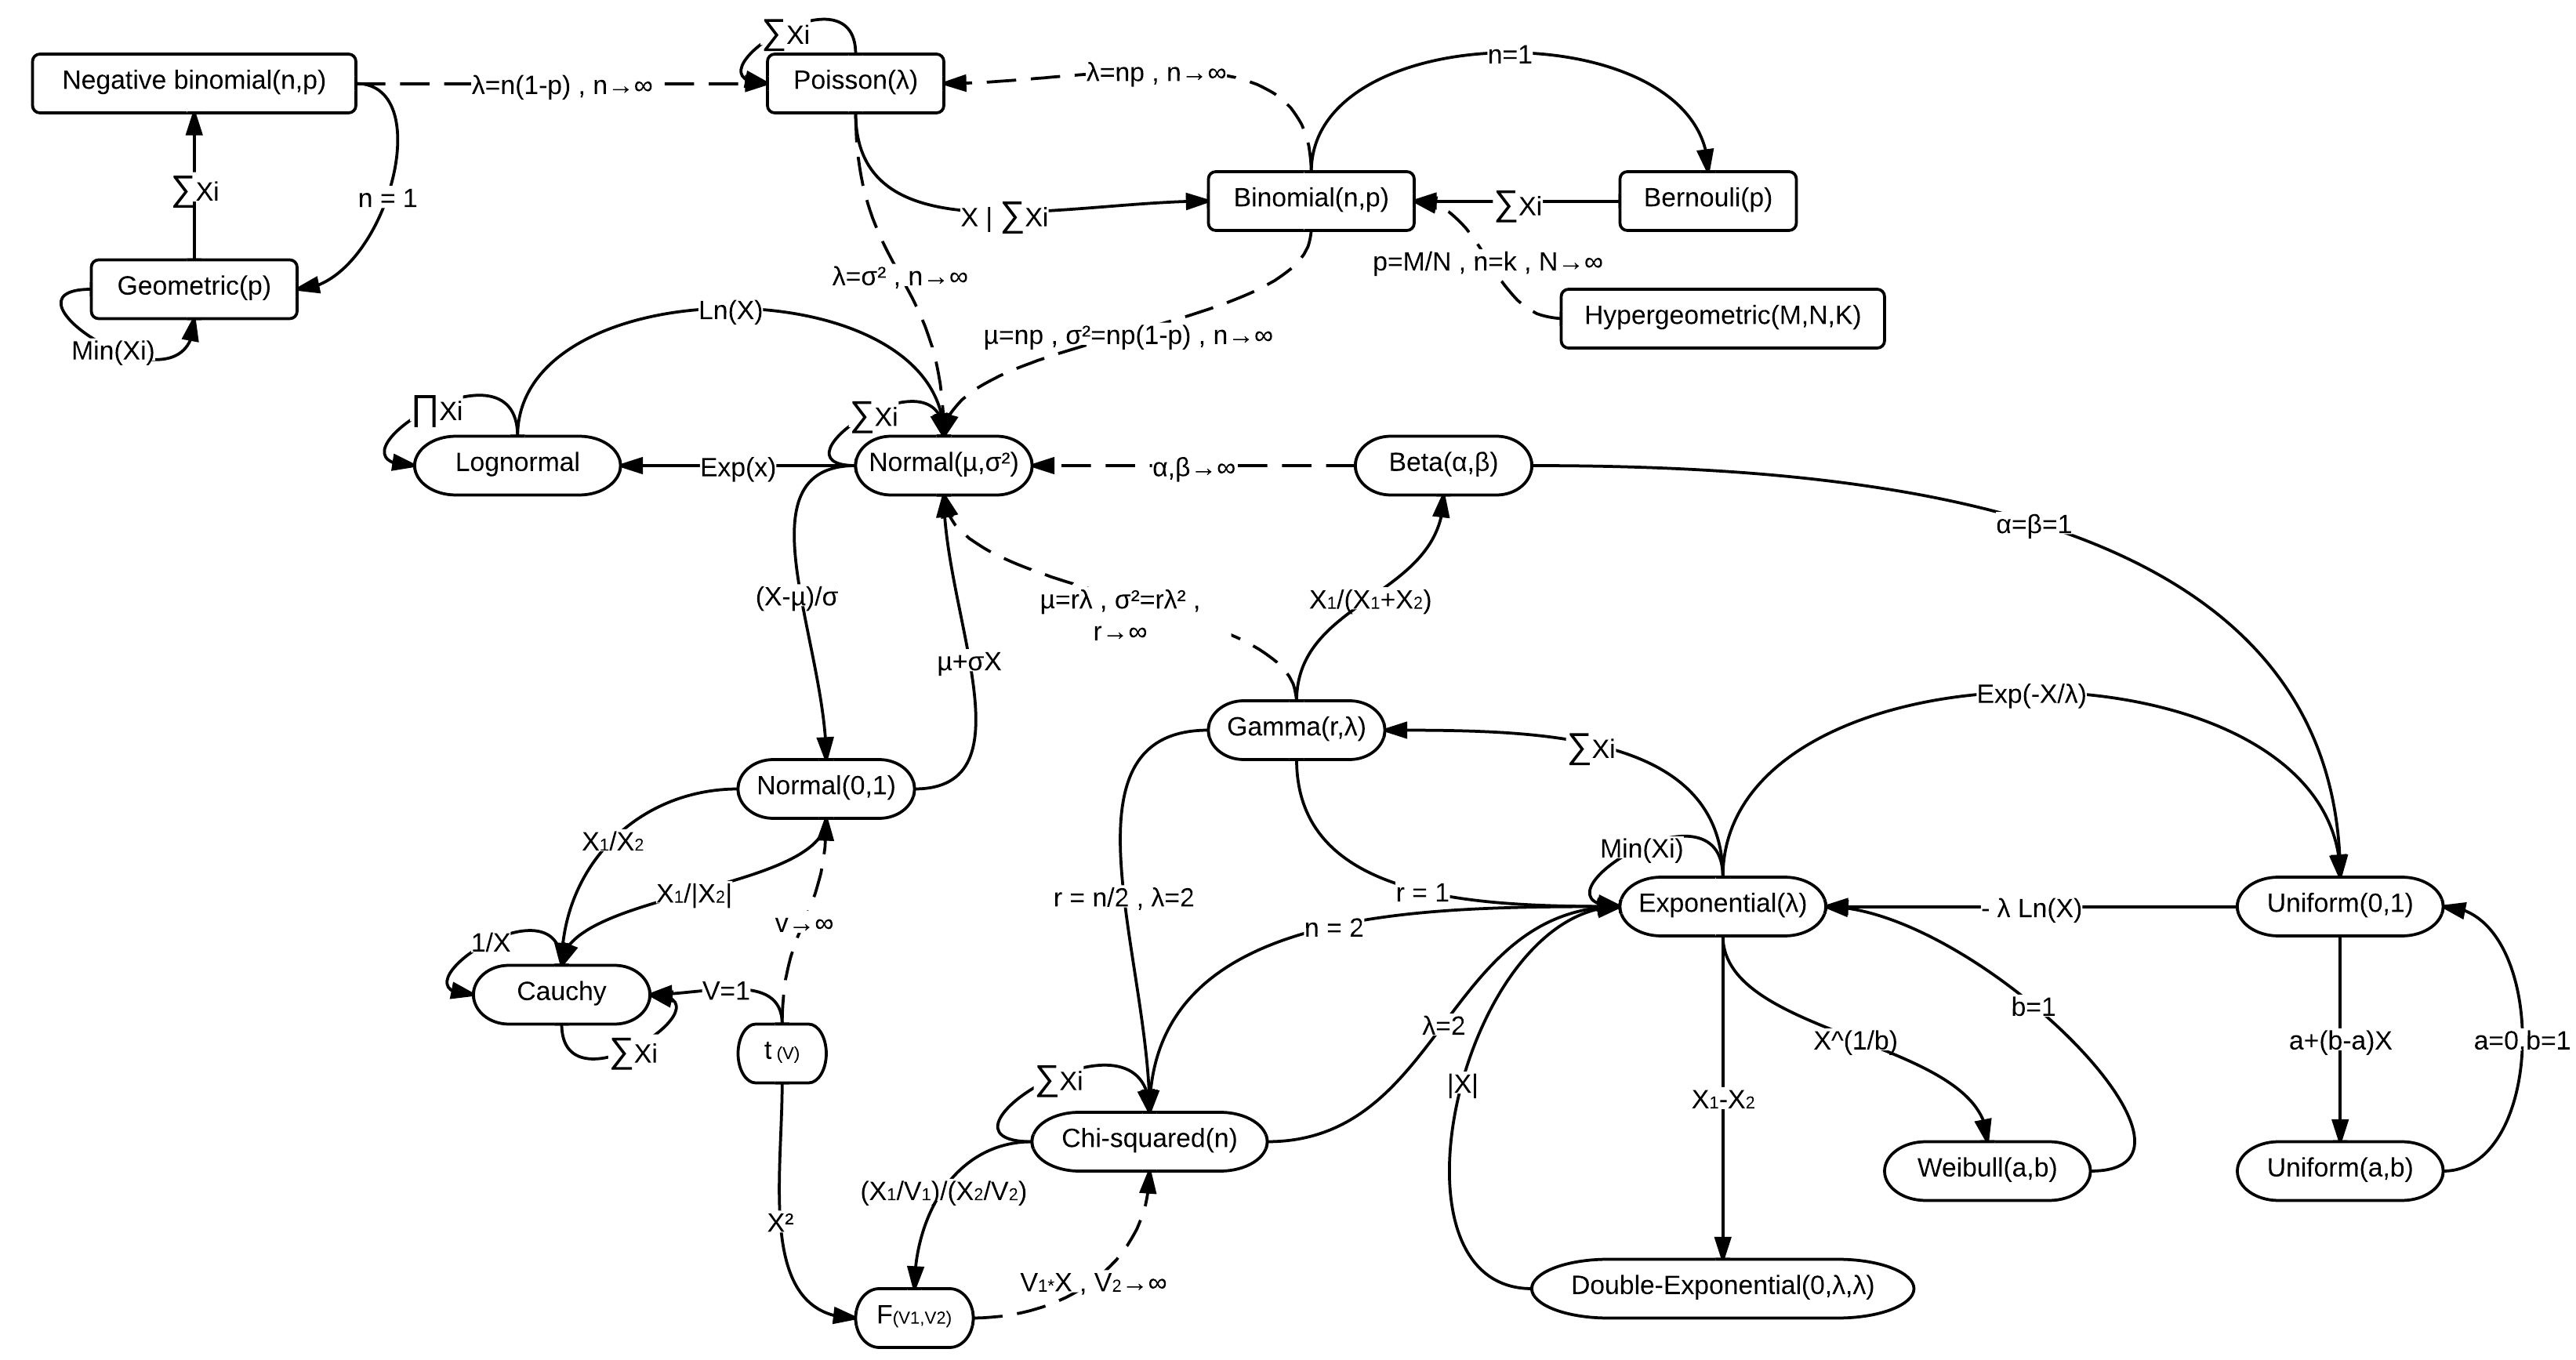
\includegraphics[width=800px]{distr_relationship_wikipedia} \end{center}

\end{document}
